\section{Data Pre-processing} (correlazioni tra variabili e esclusione variabili inutili) 
Missing values
partizionamento \\
Nel lavoro di data-preprocessing ci siamo curati di riempire i valori delle celle mancanti, eliminare le correlazioni fra le variabili  ed escludere le variabili inutili

\subsection{Missing values}
Il dataset presenta 19 valori mancanti alla voce SES e 2 alla voce MMSE. La trattazione di tali valori è stata affrontata in modo differente:
\begin{itemize}
    \item SES: qui i valori mancanti sono stati sostituiti dall'interpolazione lineare con i dati presenti dell'attributo in questione. Questo per mantenere la distribuzione dei dati piuttosto omogenea.
    \item MMSE: in questo caso le righe corrispondenti ai valori mancanti sono state scartate. Considerando che l'MMSE si basa su un questionario scritto individuale ed è quindi una variabile difficile da essere predetta sulla base dei risultati degli altri pazienti. Inoltre i record scartati sono solo due, dunque si assume non inficino visibilmente sui risultati finali.
\end{itemize}
 
\subsection{Correlazione fra le variabili}
Alcuni attributi del dataset risultano essere legati tra di loro. Vista la definizione di eTIV, nWBV e ASF un legame tra di essi sembra suggerito. Analizzando gli attributi si può notare una correlazione quasi lineare tra ASF e il volume intracranico, in quanto all'aumentare del volume intracranico diminuisce il fattore di scala. La spiegazione risiede nel fatto che aumentando il volume intracranico aumenta, di conseguenza, anche il possibile volume del cervello, causando quindi la diminuzione del fattore di scala tra il cervello del paziente e quello standard, ovvero l'ASF.
La percentuale di volume cerebrale (nWBV), invece, non risulta avere connessioni con l'ASF. Infatti la percentuale è insensibile alle variazioni di grandezza del cranio.
Le precedenti considerazioni ci portano a escludere l'attributo ASF dai modelli.

\begin{figure}[H]
    \centering
    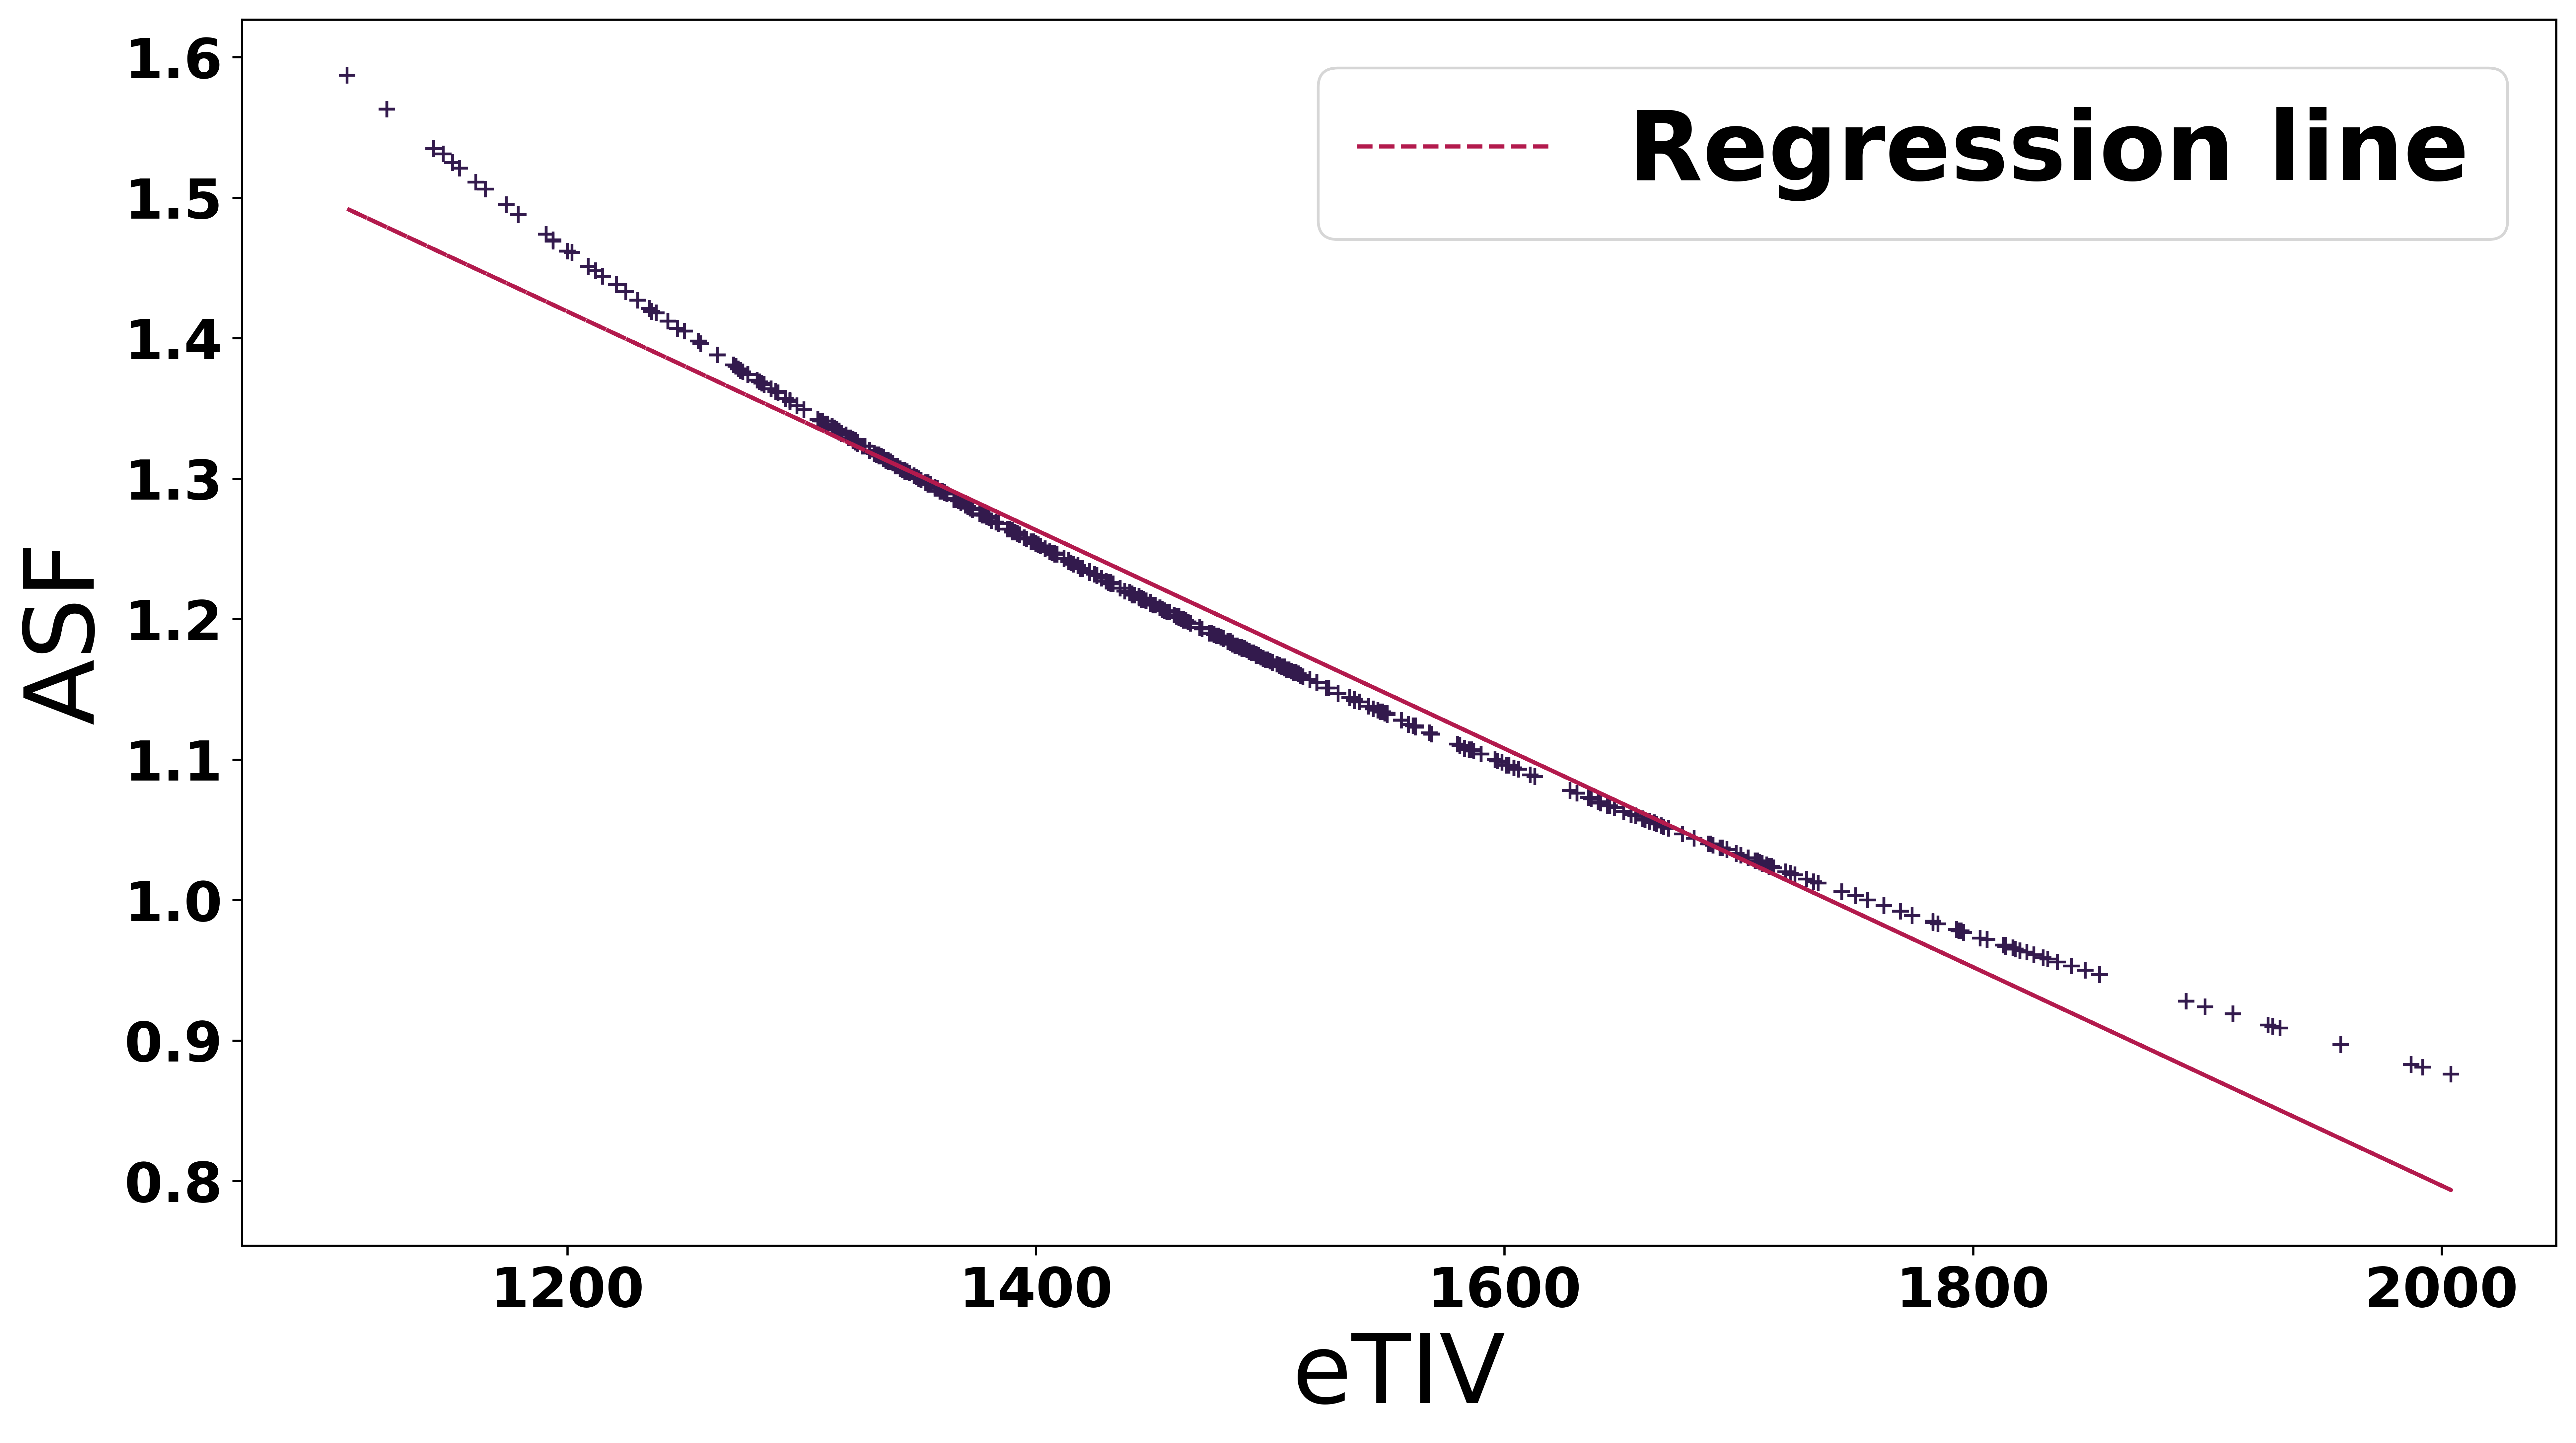
\includegraphics[height=0.55 \linewidth]{eTIV_ASF.png}
    \caption{Il grafico mostra sulle ascisse il volume intracranico (eTIV) e sulle ordinate l'Atlas Scale Factor (ASF)}
    \label{fig:conf sperimentale}
\end{figure}


%Gli unici parametri correlati sono l'eTIV e ASF. Infatti il primo restituisce il volume intracranico, il secondo il rapporto fra il cervello del paziente e il volume intracranico e il terzo rappresenta il fattore di scala fra il cervello del paziente e il cervello "standard" nell'atlante scelto. Dalla conoscenza di due fra i tre parametri possiamo quindi ricavare il terzo, per eliminare questa dipendenza scegliamo quindi di eliminare l'attributo ASF.









